\documentclass[14pt]{extbook}
\usepackage{multicol, enumerate, enumitem, hyperref, color, soul, setspace, parskip, fancyhdr} %General Packages
\usepackage{amssymb, amsthm, amsmath, bbm, latexsym, units, mathtools} %Math Packages
\everymath{\displaystyle} %All math in Display Style
% Packages with additional options
\usepackage[headsep=0.5cm,headheight=12pt, left=1 in,right= 1 in,top= 1 in,bottom= 1 in]{geometry}
\usepackage[usenames,dvipsnames]{xcolor}
\usepackage{dashrule}  % Package to use the command below to create lines between items
\newcommand{\litem}[1]{\item#1\hspace*{-1cm}\rule{\textwidth}{0.4pt}}
\pagestyle{fancy}
\lhead{Progress Quiz 4}
\chead{}
\rhead{Version C}
\lfoot{4378-7085}
\cfoot{}
\rfoot{Fall 2020}
\begin{document}

\begin{enumerate}
\litem{
Choose the equation of the function graphed below.
\begin{center}
    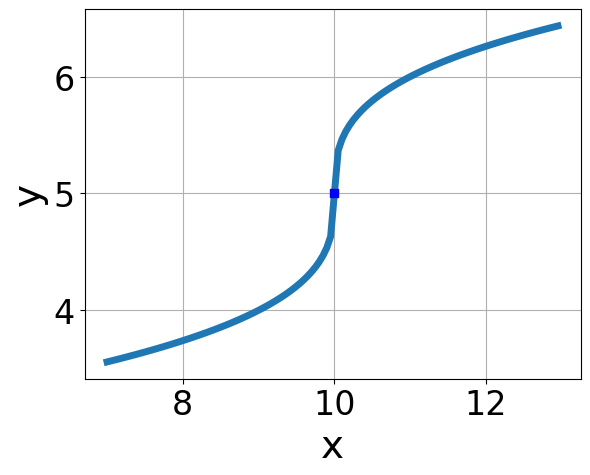
\includegraphics[width=0.5\textwidth]{../Figures/radicalGraphToEquationC.png}
\end{center}
\begin{enumerate}[label=\Alph*.]
\item \( f(x) = \sqrt[3]{x - 14} + 3 \)
\item \( f(x) = \sqrt[3]{x + 14} + 3 \)
\item \( f(x) = - \sqrt[3]{x - 14} + 3 \)
\item \( f(x) = - \sqrt[3]{x + 14} + 3 \)
\item \( \text{None of the above} \)

\end{enumerate} }
\litem{
Solve the radical equation below. Then, choose the interval(s) that the solution(s) belongs to.\[ \sqrt{-36 x^2 + 45} - \sqrt{-24 x} = 0 \]\begin{enumerate}[label=\Alph*.]
\item \( x \in [1.23,2.78] \)
\item \( \text{All solutions lead to invalid or complex values in the equation.} \)
\item \( x_1 \in [-1.04, 0.3] \text{ and } x_2 \in [-0.5,6.5] \)
\item \( x \in [-1.04,0.3] \)
\item \( x_1 \in [0.17, 1.36] \text{ and } x_2 \in [-0.5,6.5] \)

\end{enumerate} }
\litem{
Solve the radical equation below. Then, choose the interval(s) that the solution(s) belongs to.\[ \sqrt{-28 x^2 - 18} - \sqrt{50 x} = 0 \]\begin{enumerate}[label=\Alph*.]
\item \( x \in [-1.42,-0.6] \)
\item \( \text{All solutions lead to invalid or complex values in the equation.} \)
\item \( x_1 \in [0.87, 1.39] \text{ and } x_2 \in [-0.03,1.6] \)
\item \( x \in [-0.8,0.1] \)
\item \( x_1 \in [-1.42, -0.6] \text{ and } x_2 \in [-1.61,-0.24] \)

\end{enumerate} }
\litem{
What is the domain of the function below?\[ f(x) = \sqrt[5]{3 x + 8} \]\begin{enumerate}[label=\Alph*.]
\item \( \text{The domain is } (-\infty, a], \text{   where } a \in [-2.3, 0.4] \)
\item \( \text{The domain is } [a, \infty), \text{   where } a \in [-1.3, 3.4] \)
\item \( \text{The domain is } [a, \infty), \text{   where } a \in [-6.5, -1.9] \)
\item \( (-\infty, \infty) \)
\item \( \text{The domain is } (-\infty, a], \text{   where } a \in [-3.6, -1.8] \)

\end{enumerate} }
\litem{
Choose the graph of the equation below.\[ f(x) = - \sqrt{x - 12} - 5 \]\begin{enumerate}[label=\Alph*.]
\begin{multicols}{2}\item 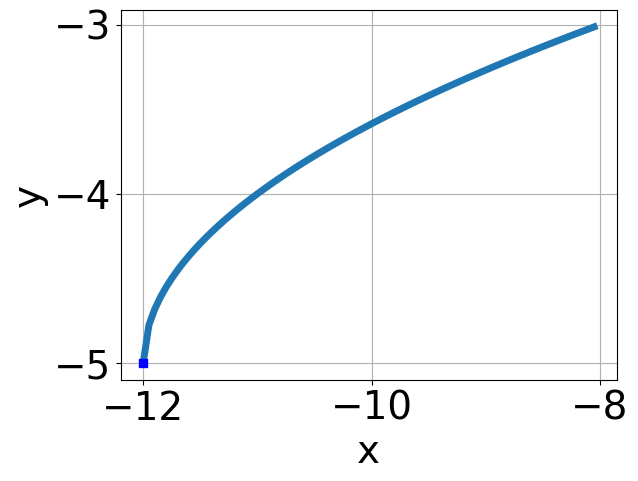
\includegraphics[width = 0.3\textwidth]{../Figures/radicalEquationToGraphAC.png}\item 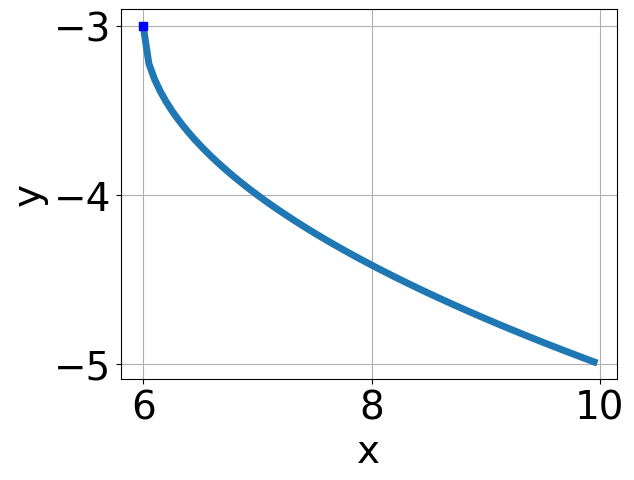
\includegraphics[width = 0.3\textwidth]{../Figures/radicalEquationToGraphBC.png}\item 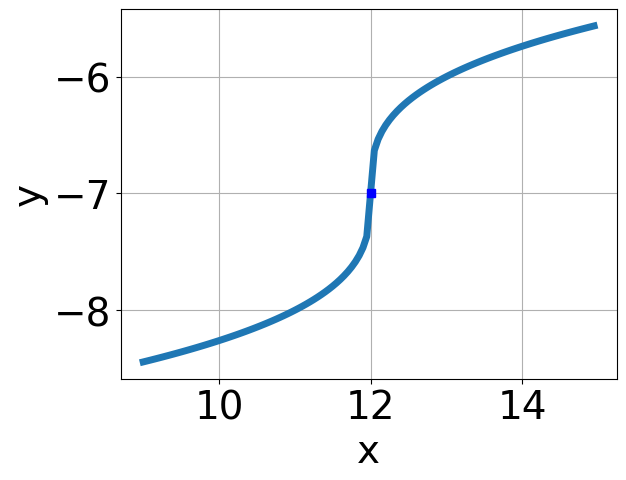
\includegraphics[width = 0.3\textwidth]{../Figures/radicalEquationToGraphCC.png}\item 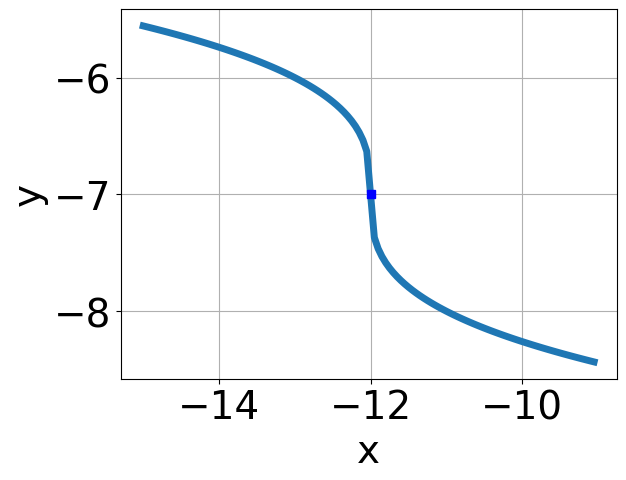
\includegraphics[width = 0.3\textwidth]{../Figures/radicalEquationToGraphDC.png}\end{multicols}\item None of the above.
\end{enumerate} }
\litem{
What is the domain of the function below?\[ f(x) = \sqrt[5]{4 x - 7} \]\begin{enumerate}[label=\Alph*.]
\item \( \text{The domain is } [a, \infty), \text{   where } a \in [0.91, 1.99] \)
\item \( (-\infty, \infty) \)
\item \( \text{The domain is } [a, \infty), \text{   where } a \in [0.55, 0.59] \)
\item \( \text{The domain is } (-\infty, a], \text{   where } a \in [-0.83, 1.04] \)
\item \( \text{The domain is } (-\infty, a], \text{   where } a \in [0.78, 2.19] \)

\end{enumerate} }
\litem{
Solve the radical equation below. Then, choose the interval(s) that the solution(s) belongs to.\[ \sqrt{-7 x + 7} - \sqrt{-9 x - 3} = 0 \]\begin{enumerate}[label=\Alph*.]
\item \( x_1 \in [-5.06, -4.58] \text{ and } x_2 \in [1,6] \)
\item \( \text{All solutions lead to invalid or complex values in the equation.} \)
\item \( x \in [-2.4,-1.6] \)
\item \( x \in [-5.06,-4.58] \)
\item \( x_1 \in [-1.35, -0.17] \text{ and } x_2 \in [1,6] \)

\end{enumerate} }
\litem{
Choose the equation of the function graphed below.
\begin{center}
    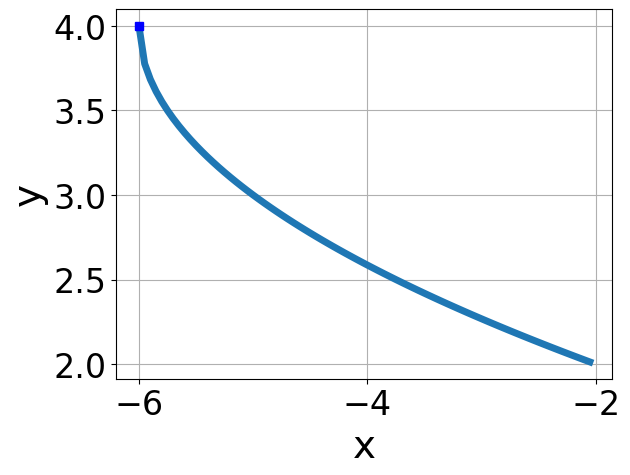
\includegraphics[width=0.5\textwidth]{../Figures/radicalGraphToEquationCopyC.png}
\end{center}
\begin{enumerate}[label=\Alph*.]
\item \( f(x) = \sqrt{x - 6} + 4 \)
\item \( f(x) = \sqrt{x + 6} + 4 \)
\item \( f(x) = - \sqrt{x - 6} + 4 \)
\item \( f(x) = - \sqrt{x + 6} + 4 \)
\item \( \text{None of the above} \)

\end{enumerate} }
\litem{
Choose the graph of the equation below.\[ f(x) = - \sqrt{x + 12} + 4 \]\begin{enumerate}[label=\Alph*.]
\begin{multicols}{2}\item 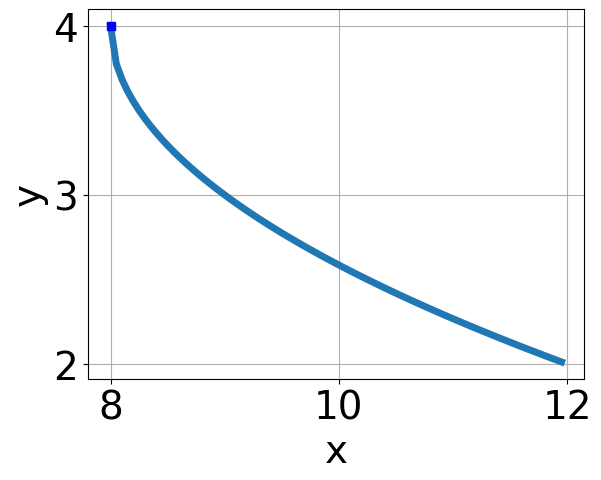
\includegraphics[width = 0.3\textwidth]{../Figures/radicalEquationToGraphCopyAC.png}\item 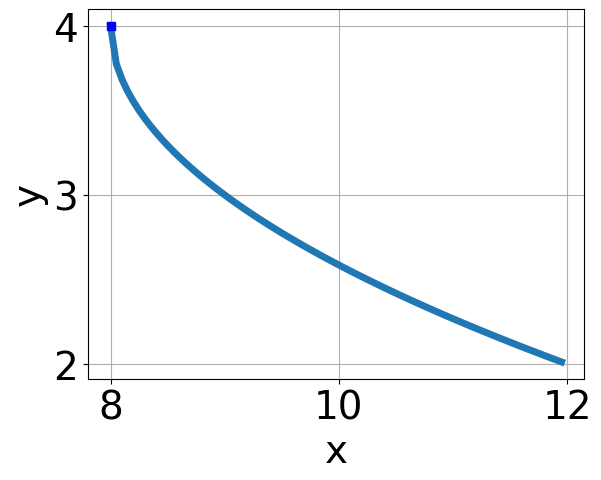
\includegraphics[width = 0.3\textwidth]{../Figures/radicalEquationToGraphCopyBC.png}\item 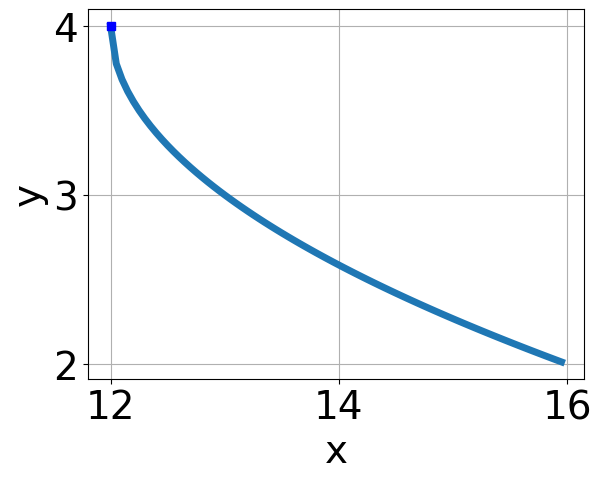
\includegraphics[width = 0.3\textwidth]{../Figures/radicalEquationToGraphCopyCC.png}\item 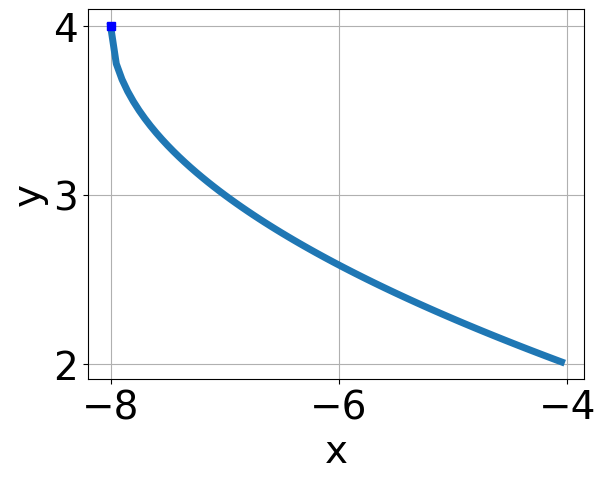
\includegraphics[width = 0.3\textwidth]{../Figures/radicalEquationToGraphCopyDC.png}\end{multicols}\item None of the above.
\end{enumerate} }
\litem{
Solve the radical equation below. Then, choose the interval(s) that the solution(s) belongs to.\[ \sqrt{-9 x - 5} - \sqrt{6 x + 5} = 0 \]\begin{enumerate}[label=\Alph*.]
\item \( \text{All solutions lead to invalid or complex values in the equation.} \)
\item \( x \in [-0.02,0.35] \)
\item \( x_1 \in [-0.69, -0.03] \text{ and } x_2 \in [-0.56,0.44] \)
\item \( x_1 \in [-1.36, -0.73] \text{ and } x_2 \in [-0.56,0.44] \)
\item \( x \in [-0.69,-0.03] \)

\end{enumerate} }
\end{enumerate}

\end{document}